\section{Verification, interpretation, and integration}
\label{sec:verification}

The proofs establish the infinite statements. The computations detect
normalization errors, compare independent finite constructions, and
illustrate the size of the proved remainders. Machine-readable outputs
are retained beside the programs that generated them.

\subsection{Exact finite checks}

The angular program verifies the first four universal degree polynomials
by symbolic coefficient extraction and supplies the rational certificate
for the derivative constant in Theorem~\ref{ang:thm:finite}.
The endpoint program compares fixed-point formal reversion with the
independent Lagrange formula \eqref{ep:eq:lagrange}; fifteen
coefficients for $q=2,3$ agree exactly. Its zero coefficients also
agree with the support restriction.

The Lambert program evaluates every factor count $1\le k\le n$
in \eqref{lm:eq:finite}, including all convolution powers through
$n=201$. The powers use the exact forward coefficient formula at
high precision, without the large-order approximation. The cases
include two positive real parameters, a generic complex parameter,
and $u=i/(2\pi)$, where $\cosh(Au/4)=0$. That last case tests
why the complex-parameter result must be additive rather than a
ratio to a possibly vanishing leading term.

\subsection{Angular numerical diagnostics}

For positive integral outer order, an independent evaluation is
\begin{equation}
 F_{a,b}(z)=\frac1{\Gamma(a)}\int_0^\infty
 t^{a-1}\Li_0(ze^{-t})\Li_b(ze^{-t})\,dt.
 \label{eq:numeric-integral}
\end{equation}
It follows by coefficientwise integration in the disk and continuation.
The program solves the angular equation using this integral and
compares the result with coefficients formed from
\eqref{ang:eq:jets}. High derivatives at the boundary use analytic
lowering, including \eqref{ang:eq:lowering}, rather than a
differentiated Fourier sum outside its convergence range. The
integral uses a precision-dependent finite upper endpoint. Its
exponentially small omitted tail is far below the displayed digits
in these diagnostics; this implementation is not an interval integrator.

At $b=1$, $\rho=1$, the displacements include
\begin{align*}
 \delta_{6,1}(1)&=0.06441843932204966951480818053626053968\ldots,\\
 \delta_{8,1}(1)&=0.02892818590626336166005258862627886175\ldots,\\
 \delta_{10,1}(1)&=0.01293779047910625463765885200102238078\ldots.
\end{align*}
The bound is designed to work simultaneously for all $b>0$ and
all radii, and is conservative near the lowest guaranteed outer
order. Table~\ref{tab:angular} displays the numerical error and
the analytic bound separately.

\begin{table}[htbp]
\centering
\caption{Degree reconstruction at $b=1$, $\rho=1$. Errors are
85-digit numerical diagnostics; bounds evaluate
\eqref{ang:eq:sum-error}.}
\label{tab:angular}
\begin{tabular}{rrrr}
\toprule
$a$ & $K$ & Numerical error & Proved upper bound \\
\midrule
6 & 4 & $1.15\times10^{-5}$ & $2.14\times10^{-1}$ \\
6 & 8 & $3.06\times10^{-8}$ & $7.05\times10^{-2}$ \\
6 & 16 & $9.24\times10^{-15}$ & $1.32\times10^{-2}$ \\
8 & 4 & $4.42\times10^{-7}$ & $7.42\times10^{-4}$ \\
8 & 8 & $8.08\times10^{-12}$ & $9.55\times10^{-6}$ \\
8 & 16 & $4.19\times10^{-19}$ & $2.72\times10^{-9}$ \\
10 & 4 & $9.79\times10^{-9}$ & $9.49\times10^{-6}$ \\
10 & 8 & $2.23\times10^{-14}$ & $4.77\times10^{-9}$ \\
10 & 16 & $1.64\times10^{-26}$ & $2.06\times10^{-15}$ \\
\bottomrule
\end{tabular}

\end{table}

For the moving construction with
$M=\lfloor(3/2)^{a/2}\rfloor$ and $K=a$, the comparison is
shown in Table~\ref{tab:moving}. The finite expression at $a=28$
has an observed error below $4\cdot10^{-61}$, while the theorem
gives the more conservative analytic bound in the last column.

\begin{table}[htbp]
\centering
\caption{Finite frequency-and-degree approximations at $b=1$,
$\rho=1$. Bounds evaluate \eqref{ang:eq:finite-error}.}
\label{tab:moving}
\begin{tabular}{rrrrr}
\toprule
$a$ & $M$ & $K$ & Numerical error & Proved upper bound \\
\midrule
20 & 57 & 20 & $6.05\times10^{-30}$ & $1.06\times10^{-16}$ \\
24 & 129 & 24 & $4.10\times10^{-44}$ & $2.01\times10^{-28}$ \\
28 & 291 & 28 & $3.88\times10^{-61}$ & $6.30\times10^{-43}$ \\
\bottomrule
\end{tabular}

\end{table}

\subsection{Lambert and endpoint diagnostics}

Table~\ref{tab:lambert} uses $D_n=nA^nC_n/(4\Gamma(n))$ and
Theorem~\ref{lm:thm:first}. Including the first correction
decreases the observed error by a further factor on the order of
$n$. The full complex-parameter record is retained in the JSON output.

\begin{table}[htbp]
\centering
\caption{Lambert coefficient diagnostics at $u=0.1$. The errors
compare the full finite formula with the leading term, and with
the leading term plus the first correction.}
\label{tab:lambert}
\begin{tabular}{rrr}
\toprule
$n$ & Leading-term error & Error with first correction \\
\midrule
40 & $1.176\times10^{-2}$ & $1.657\times10^{-3}$ \\
41 & $1.228\times10^{-2}$ & $1.525\times10^{-3}$ \\
80 & $5.430\times10^{-3}$ & $3.801\times10^{-4}$ \\
81 & $5.804\times10^{-3}$ & $3.588\times10^{-4}$ \\
200 & $2.078\times10^{-3}$ & $5.799\times10^{-5}$ \\
201 & $2.250\times10^{-3}$ & $5.556\times10^{-5}$ \\
\bottomrule
\end{tabular}

\end{table}

\begin{figure}[htbp]
\centering
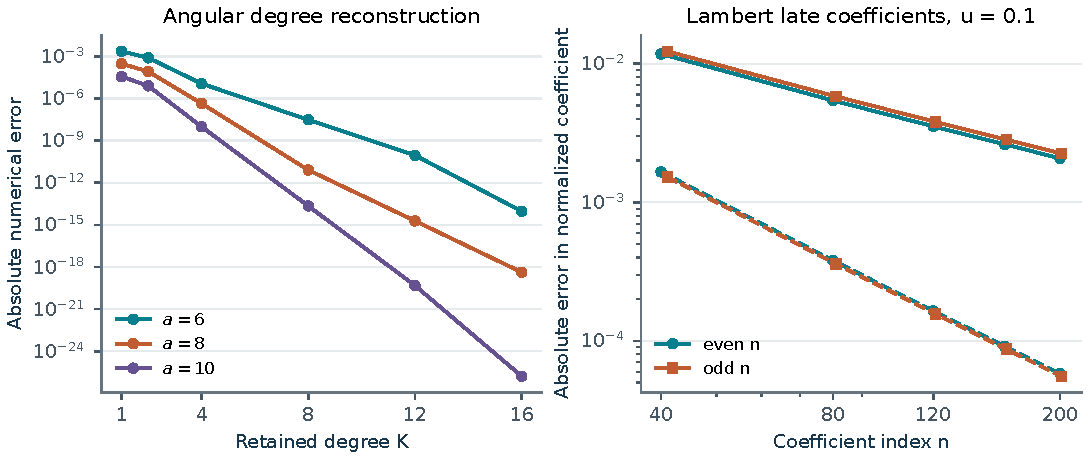
\includegraphics[width=\textwidth]{figures/diagnostics.pdf}
\caption{Numerical consequences of the proofs. Left: angular
degree reconstruction at $b=1$, $\rho=1$. Right: Lambert errors
at $u=0.1$, with even and odd indices separated. Solid curves use
the leading term; dashed curves include the first correction.
Points are diagnostics, not interval certificates.}
\label{fig:diagnostics}
\end{figure}

For the removable endpoint expansions at $y=10^{-3}$, direct
polylogarithm root calculations give polynomial errors approximately
$1.7191\cdot10^{-19}$ for \eqref{ep:eq:q2} and
$1.0461\cdot10^{-29}$ for \eqref{ep:eq:q3}. Four cut-bank tests
compare direct evaluation with an independently formed Jonqui\`ere
expansion. The local threshold is proved using exact sign estimates;
the decimals only check normalization and branch conventions.

\subsection{Recommended changes to the existing material}

No incorrect theorem was found in the particular angular finite-cutoff,
angular divergence, integer cut-modulus, or Lambert coefficient
statements used here. The justified integration changes are:
\begin{enumerate}
\item Mark the angular summation question as answered for $a\ge6$,
retaining the nonlinear-degree and radial-degree data. Preserve the
source's divergence warning.
\item Add the finite approximation as progress on moving truncation,
while keeping sharp optimality open.
\item Replace the two named Lambert conjectures with
Theorem~\ref{lm:thm:sharp}; cross-reference the first correction
and Borel decomposition. Extend the exact-radius assertion in this
model to every complex $u\ne0$.
\item Add the minimal direct-inverse ramification classification as
a refinement of the existing noninteger charts.
\item Record the failure of the all-real cut-modulus extension for
$1<s<3/2$ and the sharp local threshold. Retain the integer-order
theorem; leave both the global noninteger cut-modulus range and the
broader endpoint-circle question open.
\end{enumerate}
These are changes of mathematical status and scope. Correct historical
reports need not be rewritten, and an open question should not be
described as an erroneous theorem.

\section{Further research questions}
\label{sec:future}

\subsection{Angular summation and finite approximation}

\paragraph{1. Find the least uniform outer-order threshold.}
Determine the least $a_*$ for convergence of the scalar coupling
Taylor series at $\tau=1$, uniformly in $b>0$ and $0<\rho\le1$.
The explicit $a\ge6$ uses a simple disk and rational constants.
A sharper norm may still miss the true obstruction: a complex
coupling singularity satisfying $v=\tau f(v)$ and
$1=\tau f'(v)$, or a collision with the polylogarithm cut.

\paragraph{2. Prove a sharp optimal truncation law.}
Theorem~\ref{ang:thm:gaussian} attains every
$\lambda<\log(3/2)$ in its Gaussian exponent for one double
cutoff. Determine the sharp error for the original single
exponential-base cutoff and compare the two schemes. A lower bound
must account for the prime-frequency divergence mechanism.

\paragraph{3. Compare natural summation prescriptions.}
Compare analytic continuation in the scalar coupling, radial Abel
degree summation, and limits of exact finite-Fourier roots.
Agreement must be proved in a common domain. A summation method
depending only on coefficients already grouped by exponential base
is a separate problem because the present construction retains
additional multiset data.

\paragraph{4. Reduce the fixed period algebra.}
Use the repository's cyclotomic and depth-reduction identities to
reduce the generating set in \eqref{ang:eq:algebra}. This asks for
proved reductions, not numerical independence. Compact generator
lists could simplify many consecutive coupling coefficients.

\paragraph{5. Extend to other colors and depths.}
The local construction needs a simple dominant zero and a controlled
complex tail. Identifying it with the intended global geometric zero
requires a separate global theorem. Keep those tasks distinct when
studying other root-of-unity colors or higher-depth harmonic sums.

\subsection{Factorial reversion and Borel geometry}

\paragraph{6. Determine the full inverse Borel continuation.}
Does the inverse Borel germ continue along every path avoiding an
explicit additive action set? The log--dilog decomposition only
describes the initial disk and its boundary regularity. A continuation
theorem should separate inherited arithmetic singularities from those
created by nonlinear convolution.

\paragraph{7. Derive all relative late terms.}
The leading amplitudes detect $r_1$; the next term also detects
$r_2$ and the quadratic core. Prove exactly which finite forward
and core data determine each coefficient of $n^{-j}$ and give a
recursive formula. Borinsky's framework~\cite{Borinsky} is a
natural starting point, with the two-action parity kept explicit.
Successive terms should lead to higher polylogarithms in a refined
initial-disk decomposition.

\paragraph{8. Resolve physical moving-parameter limits.}
The physical inverse has $u=1/X$ and $q=e^{\gamma-X}$.
A useful optimal-truncation analysis must choose $n$ jointly with
$X$. Derive the transition between the action amplitudes as $u\to0$
and quantify the smallest remainder on that physical curve.

\paragraph{9. Study cancellation of a parity amplitude.}
At imaginary couplings an even or odd leading amplitude can vanish.
Classify the first nonzero late term on each such locus. The
first correction is a starting point; the cancellation of one
parity amplitude does not remove either individual logarithmic action.

\subsection{Global inverse geometry}

\paragraph{10. Determine the global cut-modulus range.}
The threshold $s=3/2$ is exact locally. For which noninteger
real $s\ge3/2$ does the strict inequality persist for every
$u>0$? Control the entire cut and distinguish the chosen
principal-sheet image boundary from intrinsic inverse singularities.

\paragraph{11. Locate the nearest singularities at exceptional orders.}
At $s=1+1/q$, $\zeta(s)$ is regular for the continued inverse,
with a critical point of order $q$. What controls the Taylor
radius of the original germ at $w=0$? Candidates include critical
values on other sheets and finite asymptotic values. The local
removability theorem does not choose among them.

\paragraph{12. Compare direct and feedback ramification.}
Seek a local classification for $\Psi(v)=\Li_s(\Phi(v))$
with prescribed vanishing orders of $\Psi$ and $\Phi-1$.
Quadratic feedback can change the direct degree $\min(p,q)$ and
create folds. Resonant logarithms must be treated separately from
rational powers; deleting them can produce a false finite-cover claim.

\paragraph{13. Formalize the reusable finite algebra.}
The finite factorial convolution inequalities, coefficient extraction,
parity formulas, and rational norm certificates are suitable first
formalization targets. Full analytic formalization also needs the
polylogarithm continuation and kernel machinery, and the relevant
complex-analytic theorems. This package makes no claim that those
prerequisites or the present proofs have already been formalized.
